% mnras_template.tex 
%
% LaTeX template for creating an MNRAS paper
%
% v3.0 released 14 May 2015
% (version numbers match those of mnras.cls)
%
% Copyright (C) Royal Astronomical Society 2015
% Authors:
% Keith T. Smith (Royal Astronomical Society)

% Change log
%
% v3.0 May 2015
%    Renamed to match the new package name
%    Version number matches mnras.cls
%    A few minor tweaks to wording
% v1.0 September 2013
%    Beta testing only - never publicly released
%    First version: a simple (ish) template for creating an MNRAS paper

%%%%%%%%%%%%%%%%%%%%%%%%%%%%%%%%%%%%%%%%%%%%%%%%%%
% Basic setup. Most papers should leave these options alone.
\documentclass[fleqn,usenatbib]{mnras}

% MNRAS is set in Times font. If you don't have this installed (most LaTeX
% installations will be fine) or prefer the old Computer Modern fonts, comment
% out the following line
\usepackage{newtxtext,newtxmath}
% Depending on your LaTeX fonts installation, you might get better results with one of these:
%\usepackage{mathptmx}
%\usepackage{txfonts}

% Use vector fonts, so it zooms properly in on-screen viewing software
% Don't change these lines unless you know what you are doing
\usepackage[T1]{fontenc}

% Allow "Thomas van Noord" and "Simon de Laguarde" and alike to be sorted by "N" and "L" etc. in the bibliography.
% Write the name in the bibliography as "\VAN{Noord}{Van}{van} Noord, Thomas"
\DeclareRobustCommand{\VAN}[3]{#2}
\let\VANthebibliography\thebibliography
\def\thebibliography{\DeclareRobustCommand{\VAN}[3]{##3}\VANthebibliography}


%%%%% AUTHORS - PLACE YOUR OWN PACKAGES HERE %%%%%

% Only include extra packages if you really need them. Common packages are:
\usepackage{graphicx}	% Including figure files
\usepackage{amsmath}	% Advanced maths commands
\usepackage{amssymb}	% Extra maths symbols

%%%%%%%%%%%%%%%%%%%%%%%%%%%%%%%%%%%%%%%%%%%%%%%%%%

%%%%% AUTHORS - PLACE YOUR OWN COMMANDS HERE %%%%%

% Please keep new commands to a minimum, and use \newcommand not \def to avoid
% overwriting existing commands. Example:
%\newcommand{\pcm}{\,cm$^{-2}$}	% per cm-squared

%%%%%%%%%%%%%%%%%%%%%%%%%%%%%%%%%%%%%%%%%%%%%%%%%%

%%%%%%%%%%%%%%%%%%% TITLE PAGE %%%%%%%%%%%%%%%%%%%

% Title of the paper, and the short title which is used in the headers.
% Keep the title short and informative.
\title[Short title, max. 45 characters]{MNRAS \LaTeXe\ template -- title goes here}

% The list of authors, and the short list which is used in the headers.
% If you need two or more lines of authors, add an extra line using \newauthor
\author[D. Neill et al.]{
Duncan Neill,$^{1}$\thanks{E-mail: dn431@bath.ac.uk}
William Newton,$^{2}$
David Tsang$^{1}$
\\
% List of institutions
$^{1}$Department of Physics, University of Bath, Claverton Down, Bath, BA1 1AL\\
$^{2}$Department of Physics and Astronomy, Texas A\&M University-Commerce, Commerce, TX, 75429-3011
}

% These dates will be filled out by the publisher
\date{Accepted XXX. Received YYY; in original form ZZZ}

% Enter the current year, for the copyright statements etc.
\pubyear{2015}

% Don't change these lines
\begin{document}
\label{firstpage}
\pagerange{\pageref{firstpage}--\pageref{lastpage}}
\maketitle

% Abstract of the paper
\begin{abstract}
We do physics and calculate stuff. 
Such Physics. Many maths. Wow.
\end{abstract}

% Select between one and six entries from the list of approved keywords.
% Don't make up new ones.
\begin{keywords}
keyword1 -- keyword2 -- keyword3
\end{keywords}

%%%%%%%%%%%%%%%%%%%%%%%%%%%%%%%%%%%%%%%%%%%%%%%%%%

%%%%%%%%%%%%%%%%% BODY OF PAPER %%%%%%%%%%%%%%%%%%

% \section{Introduction}

% This is a simple template for authors to write new MNRAS papers.
% See \texttt{mnras\_sample.tex} for a more complex example, and \texttt{mnras\_guide.tex}
% for a full user guide.

% All papers should start with an Introduction section, which sets the work
% in context, cites relevant earlier studies in the field by \citet{Fournier1901},
% and describes the problem the authors aim to solve \citep[e.g.][]{vanDijk1902}.
% Multiple citations can be joined in a simple way like \citet{deLaguarde1903, delaGuarde1904}.

% \section{Methods, Observations, Simulations etc.}

% Normally the next section describes the techniques the authors used.
% It is frequently split into subsections, such as Section~\ref{sec:maths} below.

% \subsection{Maths}
% \label{sec:maths} % used for referring to this section from elsewhere

% Simple mathematics can be inserted into the flow of the text e.g. $2\times3=6$
% or $v=220$\,km\,s$^{-1}$, but more complicated expressions should be entered
% as a numbered equation:

% \begin{align}
%     x=\frac{-b\pm\sqrt{b^2-4ac}}{2a}.
% 	\label{eq:quadratic}
% \end{align}

% Refer back to them as e.g. equation~(\ref{eq:quadratic}).

% \subsection{Figures and tables}

% Figures and tables should be placed at logical positions in the text. Don't
% worry about the exact layout, which will be handled by the publishers.

% Figures are referred to as e.g. Fig.~\ref{fig:example_figure}, and tables as
% e.g. Table~\ref{tab:example_table}.

% % Example figure
% \begin{figure}
% 	% To include a figure from a file named example.*
% 	% Allowable file formats are eps or ps if compiling using latex
% 	% or pdf, png, jpg if compiling using pdflatex
% 	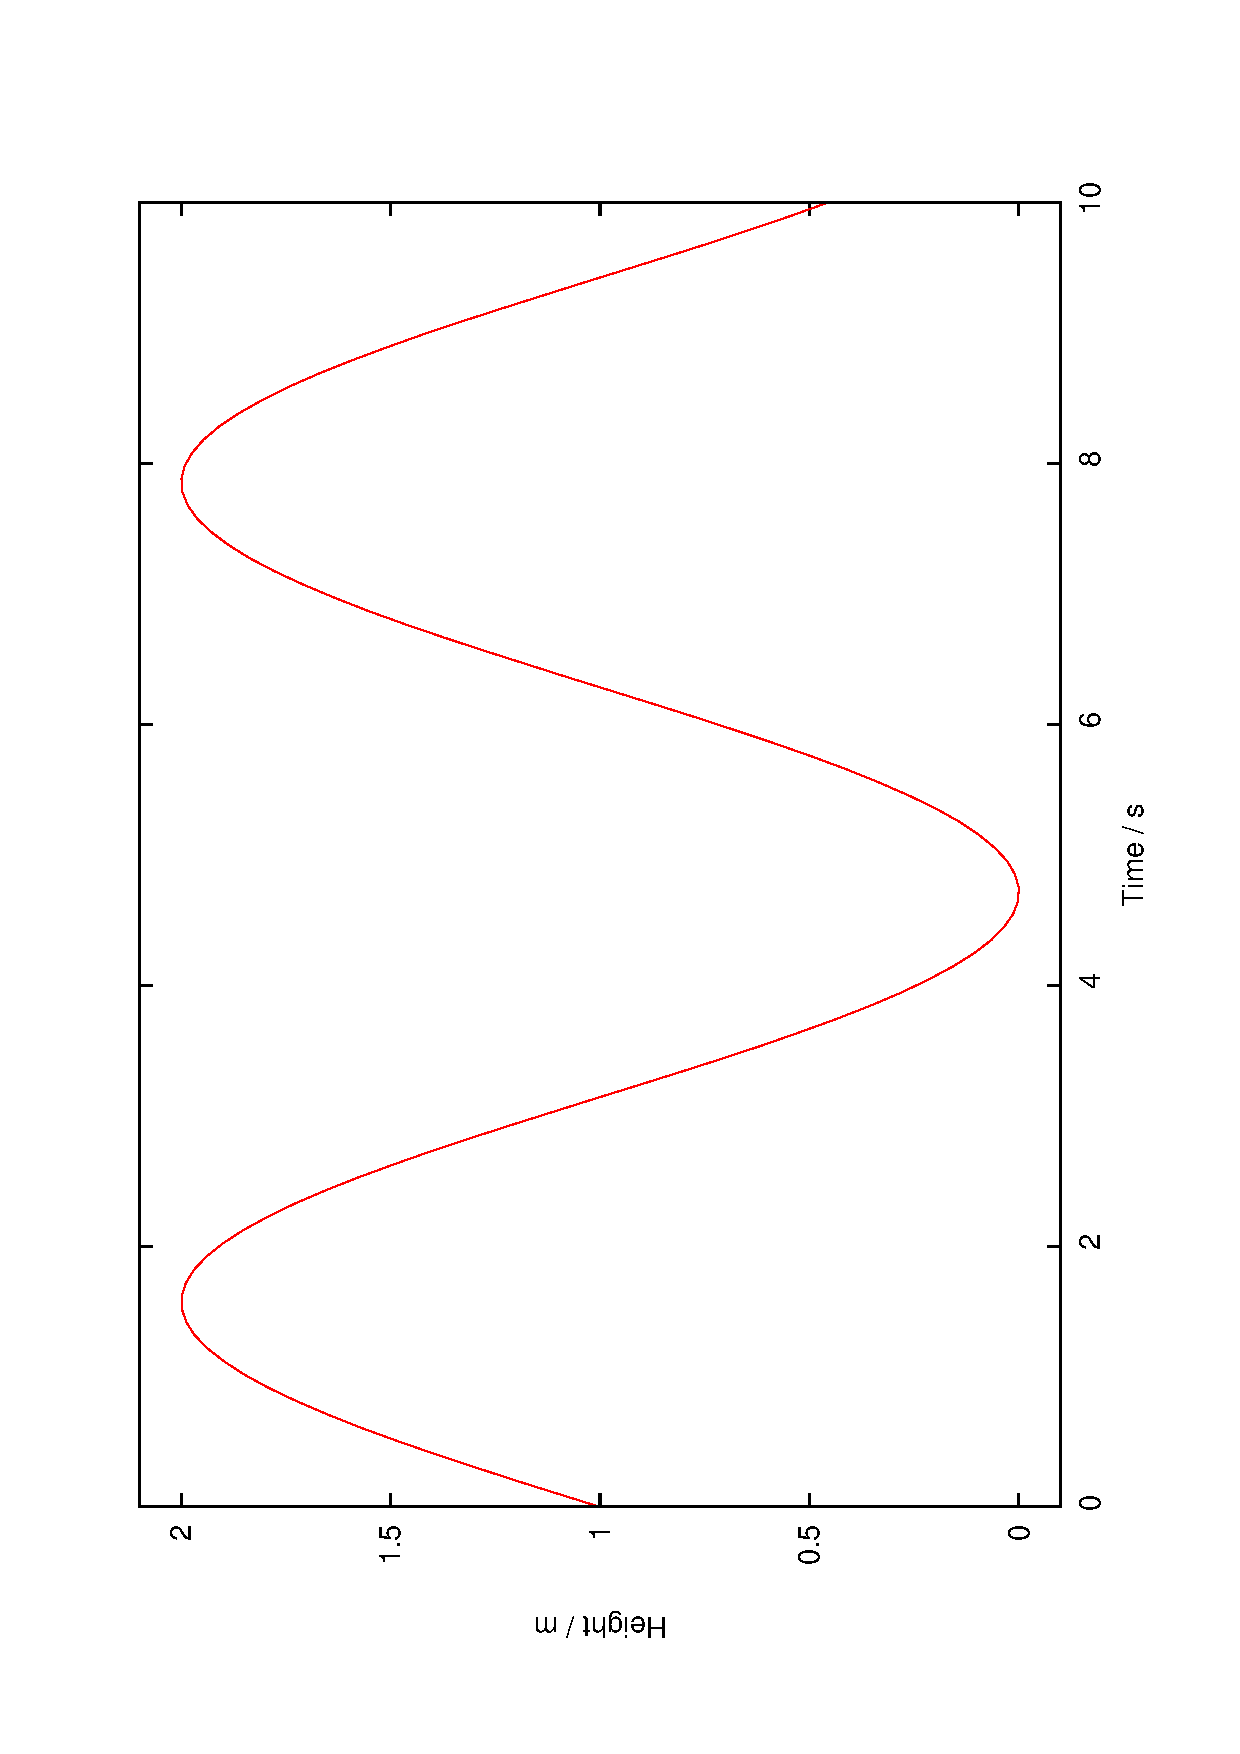
\includegraphics[width=\columnwidth]{example}
%     \caption{This is an example figure. Captions appear below each figure.
% 	Give enough detail for the reader to understand what they're looking at,
% 	but leave detailed discussion to the main body of the text.}
%     \label{fig:example_figure}
% \end{figure}

% % Example table
% \begin{table}
% 	\centering
% 	\caption{This is an example table. Captions appear above each table.
% 	Remember to define the quantities, symbols and units used.}
% 	\label{tab:example_table}
% 	\begin{tabular}{lccr} % four columns, alignment for each
% 		\hline
% 		A & B & C & D\\
% 		\hline
% 		1 & 2 & 3 & 4\\
% 		2 & 4 & 6 & 8\\
% 		3 & 5 & 7 & 9\\
% 		\hline
% 	\end{tabular}
% \end{table}


% \section{Conclusions}

% The last numbered section should briefly summarise what has been done, and describe
% the final conclusions which the authors draw from their work.

% \section*{Acknowledgements}

% The Acknowledgements section is not numbered. Here you can thank helpful
% colleagues, acknowledge funding agencies, telescopes and facilities used etc.
% Try to keep it short.

% %%%%%%%%%%%%%%%%%%%%%%%%%%%%%%%%%%%%%%%%%%%%%%%%%%
% \section*{Data Availability}

 
% The inclusion of a Data Availability Statement is a requirement for articles published in MNRAS. Data Availability Statements provide a standardised format for readers to understand the availability of data underlying the research results described in the article. The statement may refer to original data generated in the course of the study or to third-party data analysed in the article. The statement should describe and provide means of access, where possible, by linking to the data or providing the required accession numbers for the relevant databases or DOIs.


\section{Introduction}
\hspace{\parindent}Neutron stars consist of extremely dense matter, the study of which is important for our understanding of nuclear physics. To investigate the internal structure of these stars we must find ways to probe them using observational phenomena. Short gamma-ray bursts (sGRBs)~\citet{d2015short} are one such phenomena that, while their origins are uncertain, likely originate from the merging of binary neutron stars. These bursts are characterised by a large peak in the gamma-ray count that lasts for $\sim 1$ second or less. Around 10\% of sGRBs are preceded by a 'precursor' flare~\citet{troja2010precursors}. These precursor flares can be identified as a lower, separate peak in the gamma-ray count a short time ($\sim 0.1-1.0$ s) before the main peak~\citet{zhong2019precursors}. In this paper we will investigate the constraints that can be applied to nuclear physics parameters by one possible cause of precursors: resonant shattering flares.

\hspace{\parindent}In the last few years multi-messenger observations of neutron star mergers have provided insight into the origin of sGRBs. In particular, the detection of the gravitational wave signals GW170817~\citet{abbott2017merger} and GW190425~\citet{abbott2020gw190425} (which are thought to originate from mergers) has provided a new angle from which to investigate neutron stars. Here, we use the frequency of gravitational waves to investigate the possibility of a relationship between precursor flares and the normal modes within a neutron star.%second mention of how we use precursors, but have yet to actually explain what we are doing -> but the last sentence of 1st and 2nd paragraph elsewhere (at the end of the introduction?)

\hspace{\parindent}Within a star the bulk motion of matter can be described as a linear combination of an infinite set of normal modes~\citet{smeyers2011linear}. Each mode oscillates at a certain frequency, which is value that allows it to obey the boundary conditions for the displacement of matter at both the surface and core of the star. These oscillations can be driven by external gravitational fields, such as that of a binary partner. The frequency and radial profile of the modes are strongly dependant on the internal structure of the star, with different modes being dependant on different properties, such as pressure or shear forces.%mention that excitation can also occur in close encounters in globular clusters?


%define core and crust (and ocean)? or assume reader knows what they are. Might be useful for explaining that the crust has a limit to how much strain it can take.


% mention overlap integral somewhere (?)
%The amount of energy deposited in a specific mode is determined by its overlap with the tidal field, with a stronger overlap giving it more energy. 

\subsection{Resonant Shattering Flares}
\hspace{\parindent}During the gravitational-wave induced inspiral of neutron star binaries the normal modes of a neutron star can become excited by resonant tidal interactions with its binary partner. As the stars' orbits get smaller, the frequency of the orbit (and hence the gravitational wave frequency) increases. When the orbital frequency sweeps through the appropriate resonance windows, the normal modes are excited, causing the oscillations to rapidly grow in magnitude~\citep{tsang2012resonant, tsang2013shattering, lai1994resonant}.

\hspace{\parindent}If a resonant mode is sufficiently large to cause a crustal deformation that exceeds the breaking strain of the neutron star crust, the crust will fracture, depositing seismic energy into the crust. One such mode is the crust-core interface (i) mode. This mode is caused by the discontinuity in bulk material properties between the crust and core and has a strong overlap with the tidal field~\citet{tsang2012resonant}. This makes it a good candidate for the source of RSFs as less time will be needed at resonance for it to reach the elastic limit for the crust to begin to fracture. Such fractures and seismic waves continue to be driven until the crust reaches its elastic limit, causing it to shatter, scattering the seismic waves to high frequencies that are able to couple to the star's magnetic field, depositing energy into the magnetosphere and sparking a pair-photon fireball. Multiple colliding shells may be emitted over the course of the resonance window, leading to a single non-thermal burst with a duration of the resonance time, and the maximum luminosity determined by the surface magnetic field strength. % references?  %define overlap before this

\hspace{\parindent}For sufficiently strong surface magnetic field, these Resonant Shattering Flares (RSFs) can be detectable well beyond the Advanced LIGO horizon. Coincident timing of the RSF prompt emission and the gravitaitonal-wave chirp provides a precise measurement of the resonant mode frequency. Therefore, by using a nuclear model to calculate the i-mode frequency, the parameters of that model could be restricted to a range which results in mode frequencies that closely matches the observed gravitational wave frequency during the precursor flare. 

\hspace{\parindent}In this paper, we will explore the implications of a coincident multi-messenger detection of an RSF on constraining fundamental nuclear physics parameters. In particular we will explore the relationship between the i-mode frequency, neutron star structure, and the nuclear symmetry energy parameters that determines the behaviour of matter near nuclear saturation density. 







\subsection{Nuclear Symmetry Energy and Neutron Star Structure}
\hspace{\parindent}The mode frequencies are dependant on the neutron star equation of state (EoS), the relationship between the energy density and pressure inside the star. At low densities the EoS can be accurately calculated by using the properties of experimentally measured nuclei~\citet{baym1971ground}. However, at the extreme densities found in neutron stars we must rely on nuclear models to calculate the EoS, with different models giving significantly different EoSs. In order to reproduce physical results, these models are parameterised with various nuclear properties, such as the symmetry energy parameters. The nuclear symmetry energy is the average energy per nucleon required to convert symmetric nuclear matter (Z=N) into pure neutron matter (Z=0). At nuclear saturation density (the density of nucleons in a nucleus) the first three symmetry energy parameters are: the symmetry energy
\begin{align}
J=E_{\rm sym}(n_0),    
\label{eq:sym_J}
\end{align}
\noindent its first derivative 
\begin{align}
L=3n_0\frac{\partial E_{\rm sym}(n_b)}{\partial n_b}\biggr\rvert_{n_b=n_0},  
\label{eq:sym_L}
\end{align}
\noindent and its second derivative
\begin{align}
K_{\rm sym}=9n_0^2\frac{\partial^2 E_{\rm sym}(n_b)}{\partial n_b^2}\biggr\rvert_{n_b=n_0},
\label{eq:sym_K}
\end{align}
\noindent where $n_0\approx 0.16$ fm$^{-3}$ is the nuclear saturation density and $n_b$ is the baryon density.

\hspace{\parindent}To investigate the nuclear symmetry energy parameters we generated a set of EoSs spanning a reasonable range of values for $J$ ,$L$ and $K_{\rm sym}$. By calculating the mode frequencies for these EoSs we are able to find the relationship between the symmetry energy parameters and the gravitational wave frequency at which an RSF occurs.







\section{Parameterised Neutron Star Equation of State and Composition}














...

% \begin{figure}
% \centering
% 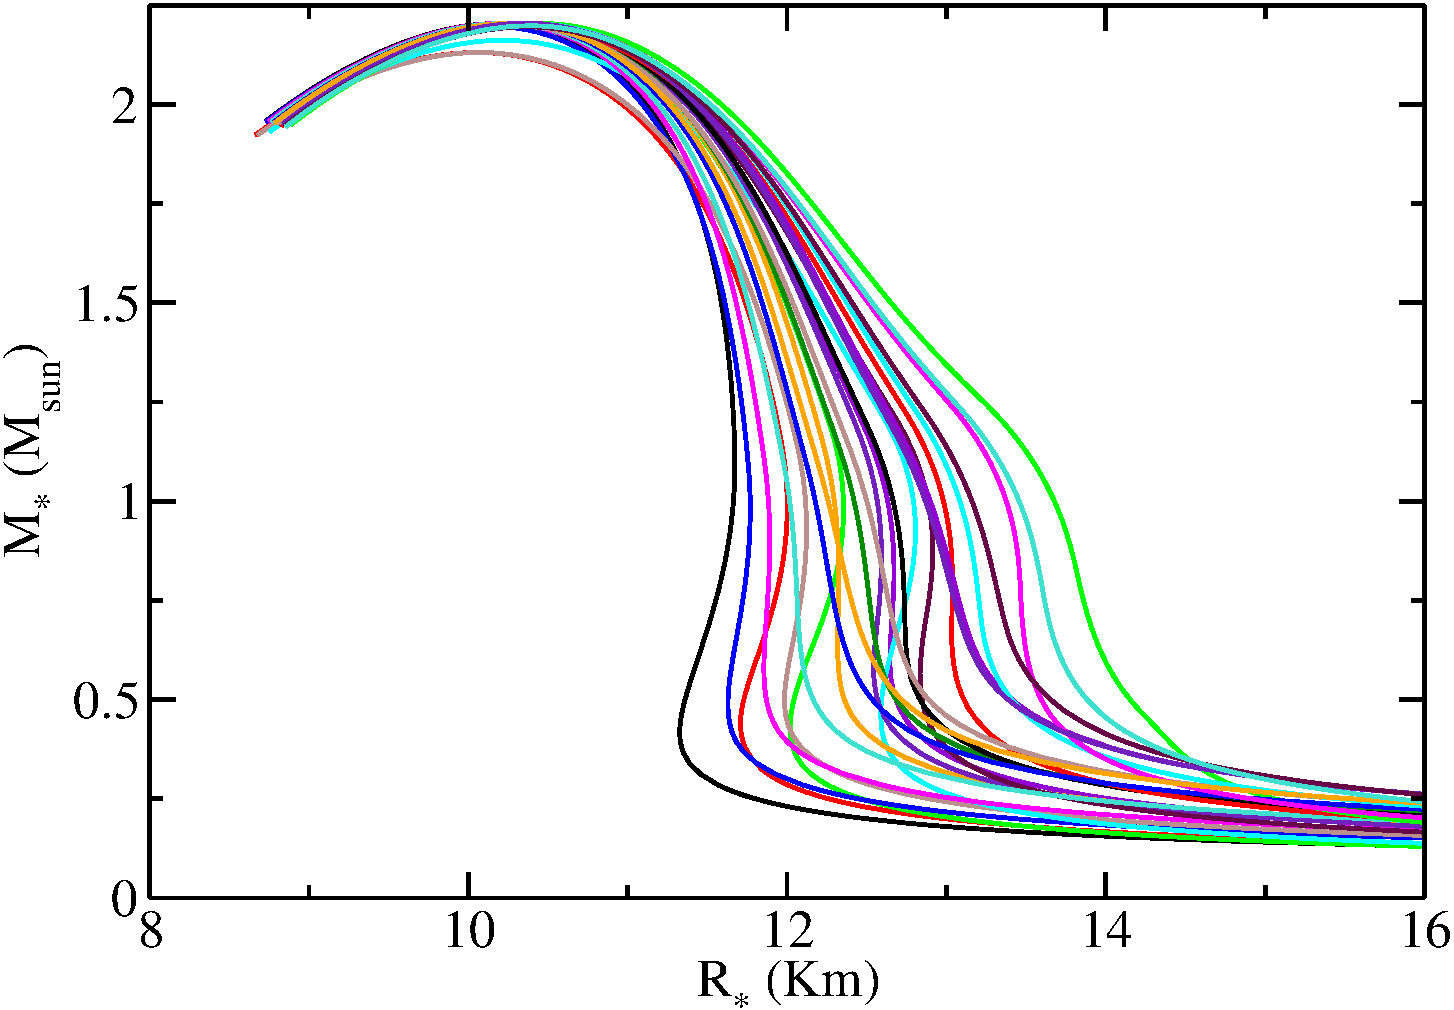
\includegraphics[width=0.45\textwidth,angle=0]{TOVs.pdf}
% \caption{The mass-radius relationships calculated using the TOV equations for all of the $J$, $L$, $K_{\rm sym}$ values.}%For EoS batch 3 (last one before the new adiabatic index calculation)
% \label{fig:TOVs}
% \end{figure}








\section{Calculation of the Normal Modes}
\hspace{\parindent}We calculate the frequencies and radial/transverse displacements of the eigenmodes of a neutron star by linearly perturbing the equations defining the equilibrium state of neutron star matter. We assume that the binary lifetime is much larger than the spin-down time of the individual neutron stars, and so we may ignore rotation and high-temperature effects. We will also assume that the frequencies of the modes that we are interested in ($\sim 10 - 100$ Hz) result in oscillations that are significantly faster than the beta-equilibrium timescale; therefore, weak-interactions do not have time to change the composition of a displaced mass element to more closely match the local composition.





\subsection{Basic Equations}
\hspace{\parindent}Following~\citet{mcdermott1988nonradial}, we begin with the equations for mass continuity, momentum conservation, and Poisson's equation:
\begin{align}
\frac{\partial\rho}{\partial t}+\nabla\cdot(\rho v)=0,
\label{eq:continuity_eqn}
\end{align}
\begin{align}
\frac{\partial v}{\partial t}=(v\cdot \nabla)v=\frac{1}{\rho}\nabla\cdot\sigma-\nabla\Phi,
\label{eq:momentum_eqn}
\end{align}
\begin{align}
\nabla^2\Phi=4\pi G\rho,
\label{eq:Poisson_eqn}
\end{align}
\noindent where $\rho$ is the energy density, $v$ is the velocity of the matter, $\sigma$ is the stress tensor, and $\Phi$ is the gravitational potential. Combining the linear perturbations of these equations (and taking the Cowling approximation by ignoring perturbations of the gravitational potential~\citet{cowling1941non}), we obtain the wave equation
\begin{align}\nonumber
&&\omega^2u=-\nabla\left(\frac{\Gamma_1 p}{\rho}\nabla\cdot u\right)-\nabla\left(\frac{1}{\rho}u\cdot\nabla p\right)-\hat{r}A\frac{\Gamma_1 p}{\rho}\nabla\cdot u\\\nonumber
&&+\frac{1}{\rho}\biggr(\nabla\left(\frac{2}{3}\mu\nabla\cdot u\right)-\left(\nabla\mu\cdot\nabla\right)u-\nabla\left(u\cdot\nabla\mu\right)\\
&&+\left(u\cdot\nabla\right)\nabla\mu-\mu\left(\nabla^2 u+\nabla\left(\nabla\cdot u\right)\right)\biggr),
\label{eq:wave_eqn}
\end{align}
where $u(x,t)$ is the Lagrangian displacement (the displacement of the mass element that is located at $x$ when $t=0$),
\begin{align}
A=\frac{1}{\rho}\frac{d\rho}{dr}-\frac{1}{\Gamma_1P}\frac{dP}{dr}
\label{eq:schwartz_descrim}
\end{align}
\noindent is the Schwarzschild discriminant, and
\begin{align}
\Gamma_1=\left(\frac{\partial\ln(P)}{\partial\ln(\rho)}\right)_s
\label{eq:adiabatic_index}
\end{align}
\noindent is the adiabatic index when the composition of the star is frozen. The non-diagonal terms of the stress tensor are given by $\sigma_{ij} = \mu \nabla_i u_j$, assuming the isotropic shear modulus $\mu$ given by \citet{strohmayer1991shear}
\begin{align}
\mu=\frac{0.1194}{1+17810\left(\frac{ak_bT}{\left(Ze\right)^2}\right)^2}\frac{n_i\left(Ze\right)^2}{a},
\label{eq:mu_1991}
\end{align}
\noindent where $T$ is the temperature, $n_i$ is the ion density, $Z$ is the proton number of the nuclei, and 
\begin{align}
a=\left(\frac{3}{4\pi n_i}\right)^{\frac{1}{3}}.
\label{eq:mu_1991_a}
\end{align}
\noindent Taking the perturbations to have time dependence of the form $e^{i\omega t}$, where $\omega$ is the mode frequency, we have 
\begin{align}
u(x,t)=\xi(x)e^{i\omega t}.
\label{eq:time_seperation}
\end{align}
\noindent In spherical coordinates this can be further separated into radial and transverse components:
\begin{align}
\xi_r=U(r)Y_{lm},\;\;\;\xi_{\theta}=V(r)\frac{\partial Y_{lm}}{\partial\theta},\;\;\;\xi_{\phi}=\frac{V(r)}{sin(\theta)}\frac{\partial Y_{lm}}{\partial\phi},
\label{eq:xi_seperation}
\end{align}
\noindent where $U(r)$ is the radial displacement, $V(r)$ is the transverse displacement, and $Y_{lm}$ are the spherical harmonics.

\hspace{\parindent}By using the separation of variables given in equations \ref{eq:time_seperation} and \ref{eq:xi_seperation}, the wave equation can be rewritten in terms of $U$ and $V$: 
\begin{align}\nonumber
&&\rho\omega^2U=\rho\frac{d\hat{\chi}}{dr}-A\Gamma_1 p\hat{\alpha}-\frac{d}{dr}\left(\frac{1}{3}\mu\hat{\alpha}\right)+\frac{d\mu}{dr}\left(\hat{\alpha}-2\frac{dU}{dr}\right)\\
&&-\mu\left(\frac{1}{r^2}\frac{d}{dr}\left( r^2\frac{dU}{dr}\right)-\frac{l(l+1)}{r^2}U+\frac{2l(l+1)}{r^2}V\right),
\label{eq:Ueqn}
\end{align}
\begin{align}\nonumber
&&\rho\omega^2V=\rho\frac{\hat{\chi}}{r}-\frac{1}{3}\frac{\mu\hat{\alpha}}{r}-\frac{d\mu}{dr}\left(\frac{dV}{dr}-\frac{V}{r}+\frac{U}{r}\right)\\
&&-\mu\left(\frac{1}{r^2}\frac{d}{dr}\left(r^2\frac{dV}{dr}\right)-\frac{l(l+1)}{r^2}V+\frac{2}{r^2}U\right),
\label{eq:Veqn}
\end{align}
% \begin{align}
% \frac{1}{r^2}\frac{d}{dr}\left(r^2\frac{d\hat{\Phi}'}{dr}\right)-\frac{l(l+1)}{r^2}\hat{\Phi}'=4\pi G\left(U\frac{d\rho}{dr}+\hat{\alpha}\rho\right),
% \label{eq:Phihat_eqn}
% \end{align}
\noindent where:
\begin{align}
\hat{\alpha}=\frac{1}{r^2}\frac{d}{dr}(r^2U)-\frac{l(l+1)}{r}V,
\label{eq:alphahat}
\end{align}
\begin{align}
\hat{\chi}=-\frac{\Gamma_1p}{\rho}\hat{\alpha}-\frac{1}{\rho}\frac{\partial p}{\partial r}U.
\label{eq:chihat}
\end{align}
%I FELL LIKE THERE SHOULD BE SOMETHING MORE HERE?








\hspace{\parindent}In this work we have applied Newtonian perturbations to a relativistic equilibrium stellar structure, resulting in a hybrid model. In order for this model to be usable, the modes must be orthogonal to properly describe the vector space of mass displacements within the star. The eigenfunction and eigenvalue of any mode can be defined in relation to the oscillation operator, $\mathcal{H}$, by \citet{reisenegger1994multipole}:
\begin{align}
\mathcal{H}\xi=-\omega^2\xi.
\end{align}
\noindent Newtonian perturbations will only result in orthogonal modes if $\mathcal{H}$ is hermitian with respect to the inner product of two vector fields (any two displacements of matter within the star), ie:
\begin{align}
\int_*\rho_0(r)\zeta^*(x)\cdot\mathcal{H}\Psi(x)d^3x=\int_*\rho_0(r)\mathcal{H}\zeta^*(x)\cdot\Psi(x)d^3x.
\end{align}
\noindent For a Newtonian stellar model, the oscillation operator is hermitian, and therefore Newtonian perturbations can be applied to it to obtain orthogonal modes. 

\hspace{\parindent}For a relativistic stellar model, the oscillation operator is not hermitian. However, this does not pose a problem for relativistic perturbations because the eigenfrequencies that they give are complex numbers, with the imaginary component arising from the damping of the mode due to the emission of gravitational waves. This imaginary component cancels out the deviation from orthogonality that arises from $\mathcal{H}$ not being hermitian, and so relativistic perturbations can be applied to a relativistic model to obtain orthogonal modes.

\hspace{\parindent} Our hybrid model can cause problems, because the background model does not give a hermitian oscillation operator and the Newtonian oscillations do not have the extra imaginary component required to cancel out the modes' deviation from orthogonality. To fix this, we follow the calculations of \citet{reisenegger1994multipole} and artificially force the oscillation operator to be hermitian by defining the gravity within the star as
\begin{align}
g=\frac{1}{\rho}\frac{dP}{dr}.
\label{eq:rel_grav}
\end{align}
\noindent This form for the gravity makes the oscillation operator hermitian within the relativistic model, and therefore we can apply Newtonian perturbations to this modified relativistic star to obtain orthogonal modes. The change to the gravity somewhat changes the properties of the modes, but only to a small degree.













\iffalse

\hspace{\parindent}For the fluid core of a neutron star, equations \ref{eq:Ueqn}-\ref{eq:chihat} are further simplified because in a fluid the shear modulus must be zero. By using $\mu=0$, and be rewriting $U$ and $V$ as the dimensionless variables
\begin{align}
y_1=\frac{U}{r},\;\;\;\;y_2=\frac{\omega^2V}{g}
\label{eq:y1y2}
\end{align}
\noindent (where $g=\frac{1}{\rho}\frac{dP}{dr}$), 
%SAY SOMETHING ABOUT REISSENEGGER
equations \ref{eq:Ueqn}-\ref{eq:chihat} can be rewritten as a pair of coupled differential equations:
\begin{align}
\left(1+\tilde{V}\right)\frac{dy_1}{dx}=\left(\frac{\tilde{V}}{\Gamma_1}-3\right)y_1+\left(\frac{l(l+1)}{c_1\Omega^2}-\frac{\tilde{V}}{\Gamma_1}\right)y_2,
\label{eq:McDy1}
\end{align}
\begin{align}
\left(1+\tilde{V}\right)\frac{dy_2}{dx}=\left(c_1\Omega^2+Ar\right)y_1+\left(1-\tilde{U}-Ar\right)y_2,
\label{eq:McDy2}
\end{align}
\noindent where the equilibrium properties of the star are: 
\begin{align}\nonumber
\tilde{U}=\frac{d\ln\left(M_r\right)}{d\ln\left(r\right)}=4\pi r^2\rho\frac{r}{M_r},\;\;\;c_1=\left(\frac{r}{R_*}\right)^3\frac{M_*}{M_r},\;\;\;\Omega^2=\frac{\omega^2R_*^3}{GM_*},
% \label{eq:eqbm_properties1}
\end{align}
\begin{align}\nonumber
\tilde{V}=-\frac{d\ln\left(P\right)}{d\ln\left(r\right)}=-\frac{G\rho M_r}{rP}\left(1+\frac{P}{\rho c^2}\right)\left(1+\frac{4\pi r^3 P}{M_r c^2}\right)\left(1-\frac{2GM_r}{rc^2}\right)^{-1},
% \label{eq:eqbm_properties2}
\end{align}



%SKIP THIS
\hspace{\parindent}For the solid crust the shear modulus is not zero, and therefore we obtain a set of four coupled differential equations:
\begin{align}
\left(1+\tilde{V}\right)\frac{dz_1}{dx}=-\left(1+2\frac{\alpha_2}{\alpha_3}\right)z_1+\frac{1}{\alpha_3}z_2+l\left(l+1\right)\frac{\alpha_2}{\alpha_3}z_3,
\label{eq:z1dr}
\end{align}
\begin{align}\nonumber
&&\left(1+\tilde{V}\right)\frac{dz_2}{dx}=\left(-\tilde{V}c_1\Omega^2-4\tilde{V}+\tilde{U}\tilde{V}+12\Gamma_1\frac{\alpha_1}{\alpha_3}\right)z_1\\\nonumber
&&+\left(\tilde{V}-4\frac{\alpha_1}{\alpha_3}\right)z_2+l\left(l+1\right)\left(\tilde{V}-6\Gamma_1\frac{\alpha_1}{\alpha_3}\right)z_3\\
&&+l\left(l+1\right)z_4,
\label{eq:z2dr}
\end{align}
\begin{align}
\left(1+\tilde{V}\right)\frac{dz_3}{dx}=-z_1+\frac{1}{\alpha_1}z_4,
\label{eq:z3dr}
\end{align}
\begin{align}\nonumber
&&\left(1+\tilde{V}\right)\frac{dz_4}{dx}= \biggr(-\tilde{V}c_1\Omega^2+\frac{2}{\alpha_3}\biggr((2l(l+1)-1)\alpha_1\alpha_2\\\nonumber
&&+2(l(l+1)-1)\alpha_1^2\biggr)\biggr)z_3\\
&&+\left(\tilde{V}-6\Gamma_1\frac{\alpha_1}{\alpha_3}\right)z_1-\frac{\alpha_2}{\alpha_3}z_2+(\tilde{V}-3)z_4,
\label{eq:z4dr}
\end{align}
\noindent where $\alpha_1=\frac{\mu}{\rho}$, $\alpha_2=\Gamma_1-\frac{2}{3}\frac{\mu}{\rho}$, $\alpha_3=\Gamma_1+\frac{4}{3}\frac{\mu}{\rho}$, and the dimensionless variables are 
\begin{align}
&z_1=\frac{U}{r},&z_2=\frac{1}{\rho}\left((\Gamma_1p-\frac{2}{3}\mu)\hat{\alpha}+2\mu\frac{dU}{dr}\right),\\
&z_3=\frac{V}{r},&z_4=\frac{\mu}{p}\left(\frac{dV}{dr}-\frac{V}{r}+\frac{U}{r}\right).
\label{eq:z1z2z3z4}
\end{align}
\noindent $z_1$ is the radial displacement, $z_2$ is proportional to the radial traction, $z_3$ is the transverse displacement, and $z_4$ is proportional to the transverse traction.

%UNTIL HERE
\fi










%Explain how we determine where Rcc is?


\hspace{\parindent}At the boundary between the solid crust and the fluid core, there are three jump conditions that must be satisfied:
\begin{align}
U\rvert_{r=R_{cc}^{+}}=U\rvert_{r=R_{cc}^{-}},
\label{eq:jump1}
\end{align}
\begin{align}
\frac{1}{\rho}\left(\lambda\hat{\alpha}+2\mu\frac{dU}{dr}\right)\biggr\rvert_{r=R_{cc}^{+}}=\tilde{V}\left(\frac{U}{r}-\frac{\omega^2V}{g}\right)\biggr\rvert_{r=R_{cc}^{-}},
\label{eq:jump2}
\end{align}
\begin{align}
\frac{\mu}{\rho}\left(\frac{dV}{dr}-\frac{V}{r}+\frac{U}{r}\right)\biggr\rvert_{r=R_{cc}^{+}}=0,
\label{eq:jump3}
\end{align}
\noindent where 
\begin{align}
\tilde{V}=-\frac{d\ln\left(P\right)}{d\ln\left(r\right)}=-\frac{G\rho M_r}{rP}\left(1+\frac{P}{\rho c^2}\right)\left(1+\frac{4\pi r^3 P}{M_r c^2}\right)\left(1-\frac{2GM_r}{rc^2}\right)^{-1},
\end{align}
\begin{align}
\lambda=\Gamma_1P-\frac{2}{3}\mu
\end{align}
\noindent is the Lam\'e coefficient, and $R_{cc}^{+}$ ($R_{cc}^{-}$) is the value at the boundary when approaching from the crust (core) of the star. The three conditions require different properties to be continuous across the crust-core boundary. The first is for the radial displacement, the second is for the pressure, and the third is for the traction (which must be zero in the fluid core). The first two jump conditions can be combined, cancelling out the arbitrary magnitude of $U$ and $V$ (which is different in the crust and the core). This gives us
\begin{align}
\frac{r}{\rho}\frac{\left(\lambda\hat{\alpha}+2\mu\frac{dU}{dr}\right)}{U}\biggr\rvert_{r=R_{cc}^{+}}=\tilde{V}\left(1-\frac{\sigma^2r}{g}\frac{V}{U}\right)\biggr\rvert_{r=R_{cc}^{-}},
\end{align}
\noindent resulting in two conditions and two eigenvalues, $\Omega$ and $V(R_*)$.


\hspace{\parindent}Every eigenmode must satisfy the boundary conditions at the centre and surface of the star. The conditions at the surface are based on the requirement that the Lagrangian pressure perturbation goes to zero at the surface:
\begin{align}
\frac{1}{\rho}\left(\lambda\hat{\alpha}+2\mu\frac{dU}{dr}\right)\biggr\rvert_{r=R_{*}}=\tilde{V}\left(\frac{\tilde{V}-c_1\Omega^2-4+\tilde{U}}{\frac{l(l+1)}{c_1\Omega^2}-\tilde{V}}+1\right)\frac{U}{r}\biggr\rvert_{r=R_{*}},
\label{eq:surface_boundary_modified_1}
\end{align}
\begin{align}
\frac{\mu}{\rho}\left(\frac{dV}{dr}-\frac{V}{r}+\frac{U}{r}\right)\biggr\rvert_{r=R_{*}}=0,
\label{eq:surface_boundary_modified_2}
\end{align}
\noindent where every quantity is evaluated at the surface of the star ($r=R_*$), and the equilibrium properties of the star are: 
\begin{align}\nonumber
\tilde{U}=\frac{d\ln\left(M_r\right)}{d\ln\left(r\right)}=4\pi r^2\rho\frac{r}{M_r},\;\;\;c_1=\left(\frac{r}{R_*}\right)^3\frac{M_*}{M_r},\;\;\;\Omega^2=\frac{\omega^2R_*^3}{GM_*}.
\end{align}
\noindent The condition at the centre of the star follows from the requirement that $U$ and $V$ be regular there:
\begin{align}
\left(\frac{c_1\Omega^2}{l}U-\frac{\sigma^2r}{g}V\right)\biggr\rvert_{r=0}=0,
\label{eq:core_condition}
\end{align}
\noindent where every quantity is evaluated at the centre of the star ($r=0$).


\hspace{\parindent}We used the shooting method to solve for the eigenvalues by choosing their initial trial values and then solving the wave equations for $\frac{dU}{dr}$ and $\frac{dV}{dr}$ to go from the central and surface boundary conditions to the crust-core transition. We then adjusted the trial eigenvalues and repeated until the jump conditions were satisfied, indicating that a mode had been found. Figure \ref{fig:trace_minima} shows the eigenvalues at which each of the jump conditions are satisfied for a specific EoS, with modes being located at the places where both conditions are satisfied.

\begin{figure}
\centering
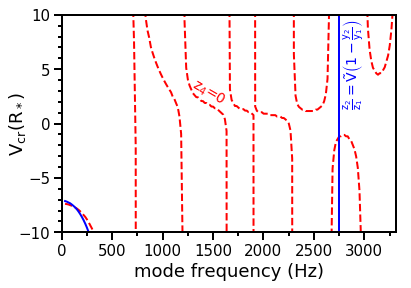
\includegraphics[width=0.45\textwidth,angle=0]{minima_30_50_-80.png}
\caption{The eigenvalues that satisfy the jump conditions at the crust-core boundary, showing the location of two modes (the interface and fundamental modes). This figure uses the EoS parameterised by $J=30$ MeV, $L=50$ MeV, and $K_{\rm sym}=-80$ MeV.}
\label{fig:trace_minima}
\end{figure}








\subsection{The Crust-Core Interface Mode}
\hspace{\parindent}Figure \ref{fig:2i_mode} shows the interface mode for one of the EoSs we have used. This mode has a distinctive peak in its radial displacement at the crust-core boundary, which is what we would expect because the i-mode is caused by the discontinuity between the crust and core. For this EoS, its eigenvalues are $\Omega=0.0805$ and $V(R_*)=-7.72$ (as can be seen in figure \ref{fig:trace_minima}), giving the mode a frequency of $134.3$ Hz. The transverse displacement in the core is small, while in the crust it discontinuously jumps to become large. This makes the i-mode a good candidate for an RSF because more of its energy will go into deforming the crust, helping it to reach the breaking strain faster.

\begin{figure}
\centering
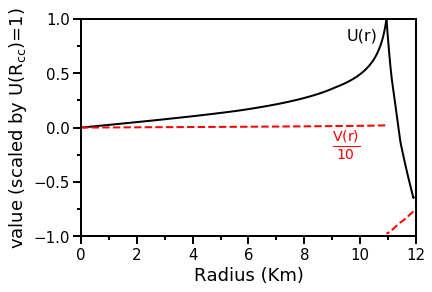
\includegraphics[width=0.45\textwidth,angle=0]{2i2_30_50_-80.png}
\caption{The $l=2$ i mode for the EoS parameterised by $J=30$ MeV, $L=50$ MeV, and $K_{\rm sym}=-80$ MeV. $V(r)$ has been reduced by an order of magnitude so that it can be plotted alongside $U(r)$.}
\label{fig:2i_mode}
\end{figure}

\hspace{\parindent}The i-mode has a strong dependence on the shear modulus in the crust, and more specifically at the crust-core transition. We investigated this dependence by considering a shear modulus scaled by 
\begin{align}
\tilde{\mu} = B \mu,
\end{align}
\noindent where the constant $B$ was varied to determine its impact on the i-mode. Figure \ref{fig:mu_B} shows the relationship between $B$ and the i-mode frequency. The constant which controls the scaling due to temperature was not varied because we have assumed that the temperature of the star is low and therefore this constant would need to be very large to have a noticeable impact on the shear modulus. Modifying the shear modulus by varying $B$ is very artificial because it is strongly linked to the other equilibrium properties of the star, and so they would also have to be changed to realistically modify the shear modulus. Therefore, changing the shear modulus in this way should only be seen as a rough guide to its impact on the frequency.

\begin{figure}
\centering
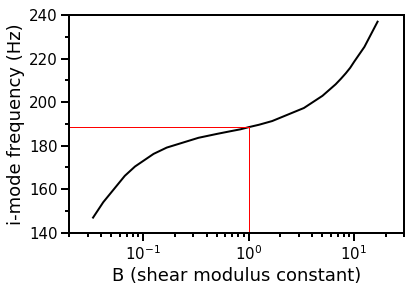
\includegraphics[width=0.45\textwidth,angle=0]{B_vs_f.png}
\caption{The change in i-mode frequency caused by scaling the shear modulus with a constant. The red lines indicate the result for $B=1$ (which gives equation \ref{eq:mu_1991}).}
\label{fig:mu_B}
\end{figure}









\section{Results}
\hspace{\parindent}Figure \ref{fig:f_vs_R_varyJ} shows the relationship between the frequency of the i-mode and both the location of the crust-core transition and the total radius of the star for EoSs with various $J$ values. Figures \ref{fig:f_vs_R_varyL} and \ref{fig:f_vs_R_varyK} show the same, but for various $L$ and $K_{\rm sym}$ values. This figure was created by using the TOV equations to find $R_*$ and $R_{cc}$ for neutron stars with masses between $0.8$ and $2.0$ M$_{\odot}$, and then calculating the i-mode frequency for each of the stars. The $J$ and $L$ values were varied to see how they affect the i-mode and radius of the star. From this we can see that the frequency increases with $J$, $K_{\rm sym}$, and (most of the time) $R_*$. It decreases with $L$ and $M_*$ (which itself decreases with increasing $R_*$), and switches from increasing to decreasing with $R_{cc}$ around $1.4$ M$_{\odot}$.
% what can we learn from this figure? (relationship to the bulk properties M* and R*?)

\begin{figure}
\centering
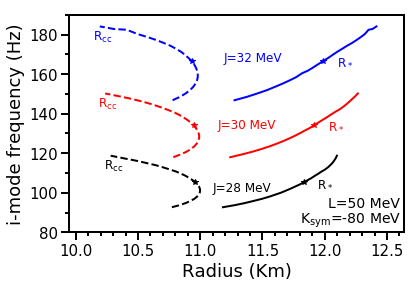
\includegraphics[width=0.45\textwidth,angle=0]{f_Rcc_Rstar_J_grid.png}
\caption{The relationship between neutron star radius and i-mode frequency. The figure shows both the total radius (solid lines) and crust-core radius (dashed lines) for each frequency. The stars indicate $1.4$ solar mass neutron stars. Increasing total radius causes the central pressure and total mass to decrease, with each line showing the change in frequency and radius between $0.8$ and $2.0$ solar masses. The three different colours are for three different $J$ values, all of which use $L=50$ MeV and $K_{\rm sym}=-80$ MeV.}
\label{fig:f_vs_R_varyJ}
\end{figure}

\begin{figure}
\centering
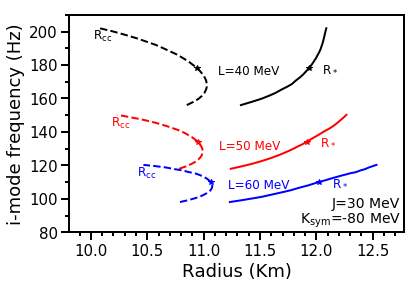
\includegraphics[width=0.45\textwidth,angle=0]{f_Rcc_Rstar_L_grid.png}
\caption{The same as figure \ref{fig:f_vs_R_varyJ}, but the three different colours are for three different $L$ values, all of which use $J=30$ MeV and $K_{\rm sym}=-80$ MeV. The red (middle) lines are the same for both figures.}
\label{fig:f_vs_R_varyL}
\end{figure}

\begin{figure}
\centering
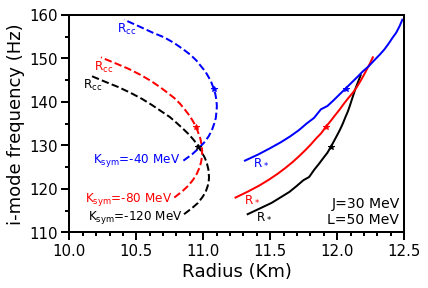
\includegraphics[width=0.45\textwidth,angle=0]{f_Rcc_Rstar_K_grid.png}
\caption{The same as figure \ref{fig:f_vs_R_varyJ}, but the different colours are for different $K_{\rm sym}$ values, all of which use $J=30$ MeV and $L=50$ MeV. The red lines are the same for all three figures.}
\label{fig:f_vs_R_varyK}
\end{figure}
















\subsection{Interface Mode dependence on Nuclear Parameters}
\hspace{\parindent}Unless otherwise stated, our results are for $1.4M_{\odot}$ neutron stars. The ranges of the symmetry energy parameters for the first set of EoSs that we used were $25\leq J\leq 35$ MeV, $20\leq L\leq 80$ MeV, and $-200\leq K_{\rm sym}\leq 40$ MeV. These ranges were chosen to confidently cover the ranges predicted by other works~\cite{liu2010nuclear,tsang2012constraints,lattimer2013constraining,balantekin2014nuclear}, and so they are very conservative. We interpolated between the i-mode frequencies for these EoSs to find surfaces of constant frequency in the $J$,$L$,$K_{\rm sym}$ parameter space, shown in figure \ref{fig:grid_J_L_K}. 




\begin{figure}
\centering
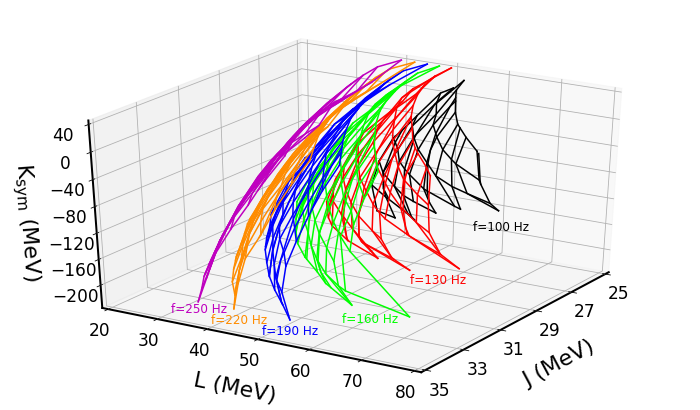
\includegraphics[width=0.45\textwidth,angle=0]{grid_J_L_K.png}
\caption{Surfaces of constant i-mode frequency in the $J$,$L$,$K_{\rm sym}$ parameter space for a wide range of symmetry energy parameter values.}
\label{fig:grid_J_L_K}
\end{figure}





Figure \ref{fig:J_vs_L_vs_f+tc} shows how the frequency changes with $J$ and $L$ for $K_{\rm sym}=-80$ MeV. The time before the merger ($t_c-t$) is related to the chirp mass and the gravitational wave frequency by \citep{blanchet2006gravitational} %check this ref. is okay
\begin{align}
t_c-t=\frac{3}{8}t_{GW}=1.76\times 10^{-3}\rm{s}\left(\frac{\mathcal{M}}{1.2M_{\odot}}\right)^{-\frac{5}{3}}\left(\frac{f_{GW}}{1000 \rm{Hz}}\right)^{-\frac{8}{3}}.
\label{eq:t_before_merger}
\end{align}
\noindent We then interpolated between the EoSs to obtain frequency contours in the $J,L$ plane, which are shown in figure \ref{fig:freq_contours}. From this we see that the frequency always increases with increasing $J$ and decreasing $L$, and that changes in $L$ have larger impacts on the the i-mode frequency than changes in $J$. This is what we would expect because the matter in neutron stars is highly asymmetric.
%ADD ANOTHER CONTOUR PLOT FOR HIGHER K_sym


\begin{figure}
\centering
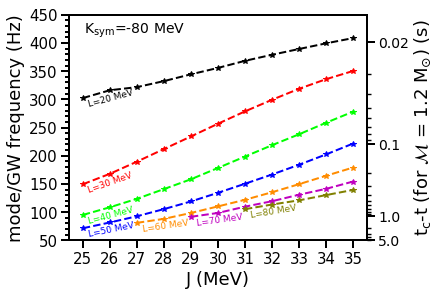
\includegraphics[width=0.45\textwidth,angle=0]{J_L_f_tc_K-80.png}
\caption{The frequency of the i-modes for various $J$ and $L$ values, and $K_{\rm sym}=-80$ MeV. On the right axis of the plot are the times before the merger at which the frequencies occur. The dotted lines connect EoSs with the same $L$ values.}
\label{fig:J_vs_L_vs_f+tc}
\end{figure}

\begin{figure}
\centering
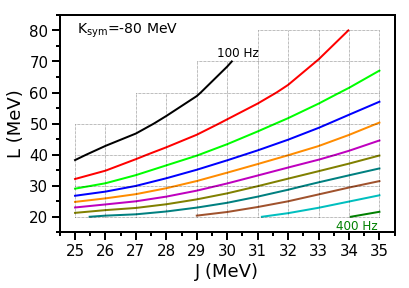
\includegraphics[width=0.45\textwidth,angle=0]{J_L_contour_K-80.png}
\caption{Frequency contours in the $J,L$ plane for $K_{\rm sym}=-80$ MeV. The gaps between the contours are $30$ Hz, and the outermost contours are labelled. The grid points indicate the results of the EoSs, between which the frequency was interpolated.}
\label{fig:freq_contours}
\end{figure}




%Other K values?
%JK plane? LK plane?

















\subsection{Constraining $J$, $L$, and $K_{\rm sym}$ with an RSF detection}
\hspace{\parindent}The timescale over which resonant excitation of a mode can occur is calculated as \citet{tsang2012resonant}
\begin{align}
t_{\rm res}\sim 8\times10^{-2}\text{s}\left(\frac{\mathcal{M}}{1.2\text{M}_{\odot}}\right)^{\frac{-5}{6}}\left(\frac{f_{\rm mode}}{100 \text{ Hz}}\right)^{\frac{-11}{6}},
\label{res_timescale}    
\end{align}
\noindent where $\mathcal{M}=\frac{M_1^{\frac{3}{5}}M_2^{\frac{3}{5}}}{(M_1+M_2)^{\frac{1}{5}}}$ is the chirp mass. This can be combined with the rate of change of the gravitational wave frequency
\begin{align}
\Dot{f}_{\rm gw}=\frac{f_{\rm gw}}{4.7\times10^{-3}\text{s}}\left(\frac{\mathcal{M}}{1.2\text{M}_{\odot}}\right)^{\frac{5}{3}}\left(\frac{f_{\rm gw}}{1000 \text{ Hz}}\right)^{\frac{8}{3}},
\label{res_timescale}    
\end{align}
\noindent where $f_{\rm gw}\approx f_{\rm mode}$. This gives a simple estimate of the range of frequencies over which resonance can occur:
\begin{align}
\delta f\sim t_{\rm res}\Dot{f}_{\rm gw}\sim3.7\text{Hz}\left(\frac{\mathcal{M}}{1.2\text{M}_{\odot}}\right)^{\frac{5}{6}}\left(\frac{f_{\rm mode}}{100 \text{ Hz}}\right)^{\frac{11}{6}}.
\label{res_timescale}    
\end{align}
\noindent From this we see that the resonance window gets larger as the frequency increases, with $\delta f$ scaling as $f_{\rm mode}^{\frac{11}{6}}$. For a chirp mass of $1.2M_{\odot}$ and a resonance at $100$ Hz, we get a frequency range of $\delta f\sim 3.7$ Hz, and for a resonance at $160$ Hz we get a range of $\delta f\sim 8.8$ Hz. This means that the spread of the frequency contours in the $J,L$ plane (which is shown in figure \ref{fig:t_res_spread}) is quite small ($\delta L\lesssim 5$ MeV), and therefore the impact of the resonance window is significantly less than that of the $K_{\rm sym}$ range, which causes a spread of around $\sim 20$ MeV in $L$ at any given $J$ value (as can be seen from how the contours change between the three plots of figure \ref{fig:freq_contours}). It should be noted that this is a very conservative estimate, and that by more accurately calculating both the rate at which energy is transferred into the modes and the breaking strain of the crust, this uncertainty could be significantly reduced by calculating the time it takes for the crust to shatter.



\begin{figure}
\centering
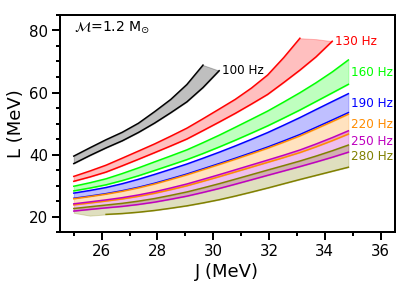
\includegraphics[width=0.45\textwidth,angle=0]{JL_spread_due_to_df_grid_nonucl.png}
\caption{Frequency contours in the $J,L$ plane for $K_{\rm sym}=-80$ MeV that have been spread by the resonance window.}
\label{fig:t_res_spread}
\end{figure}

\hspace{\parindent}Figure \ref{fig:M_vs_f} shows that neutron stars with different masses will have different i-mode frequencies, with more massive stars having lower frequencies. This means that, for a specific star, the i-mode frequency will have some degree of uncertainty propagated from the uncertainty in its mass measurement. Figure \ref{fig:vary_mass_contours} shows an example of how this uncertainty affects the $J,L$ constraints. In order to get a reasonable range for the mass uncertainty, the mass values used were taken from the low spin ranges for the stars in GW170817~\citet{abbott2017merger}. The difference between the contours' $L$ values at any given $J$ value is $0.7-2.3$ MeV. Improved measurements of NS mass would help to reduce this uncertainty, giving us a better constraint.

\begin{figure}
\centering
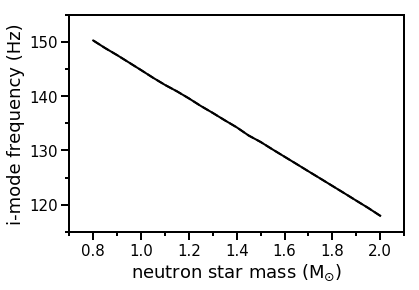
\includegraphics[width=0.45\textwidth,angle=0]{M_vs_f_30_50_-80.png}
\caption{The relationship between NS mass and the i-mode frequency for $J=30$ MeV, $L=50$ MeV, and $K_{\rm sym}=-80$ MeV.}
\label{fig:M_vs_f}
\end{figure}

\begin{figure}
\centering
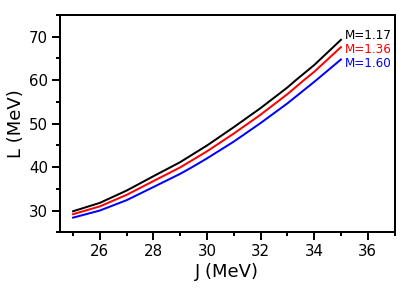
\includegraphics[width=0.45\textwidth,angle=0]{Mcomp_f160_30_50_-80.png}
\caption{The effect of changing the total NS mass on the symmetry energy parameters that give a frequency of $160$ Hz for $K_{\rm sym}=-80$ MeV.}
\label{fig:vary_mass_contours}
\end{figure}





%%%%%%%%%%%%%%%%%%%%%%%%%%%%%%%%%%


\section{Discussion}
%first sentence is repeated. I think it fits better here, so remove/change the earlier occurrence.
\hspace{\parindent}Far from symmetry we would expect higher order symmetry energy parameters ($L$, $K_{\rm sym}$) to have a stronger impact on the frequency than lower order terms ($J$). From figure \ref{fig:freq_contours} this does seem to be the case, with the contours covering a wide range of $J$ values and a smaller range of $L$ values. $K_{\rm sym}$ also has a significant impact on the i-mode frequencies, with the extremes of our $K_{\rm sym}$ range having a difference of $\Delta L\sim 20$ MeV for the same $J$ values. Figure \ref{fig:constraints} shows contours for supposed detections of RSFs at several different frequencies, with the ranges for each frequency showing the effect of the $K_{\rm sym}$ range. We would expect the frequency of a precursor flare to be $\sim 100-150$ Hz, because precursor flares tend to occur roughly half a second before the merger~\citet{zhong2019precursors}, and half a second before the merger, the frequency of GW170817 was $\sim 100-150$ Hz~\citet{abbott2017merger}.

\hspace{\parindent}....................................







\subsection{Comparisons to other constraints}
\hspace{\parindent}There are many different constraints on the symmetry energy parameters that can be found from various properties of nuclei, such as the their masses~\citet{kortelainen2010nuclear} and neutron skins~\citet{chen2010density}. By plotting these constraints together, the symmetry energy parameters $J$ and $L$ can be constrained to a small range of values~\citet{balantekin2014nuclear}. This range is shown in figure \ref{fig:constraints} alongside the contours for RSFs at several different frequencies. From this figure we see that for an i-mode frequency of $160$ Hz, our constraint has a similar $L$ uncertainty as the nuclear constraints, and so a detection at this value would help provide evidence the currently known constraints on $J$ and $L$. However, for an i-mode frequency of $200$ Hz, the constraint is shifted to significantly lower L values and therefore a detection of a precursor at $200$ Hz would improve the previous constraints on $J$ and $L$ because of the smaller overlap with the nuclear constraints. %Cite Lattimer and mention that the dipole polarisability is wrong?
% on the graph of constraints in the J,L plane, my results are similar to those for dipole polarisability
% constrain K using the J,L values?

\begin{figure}
\centering
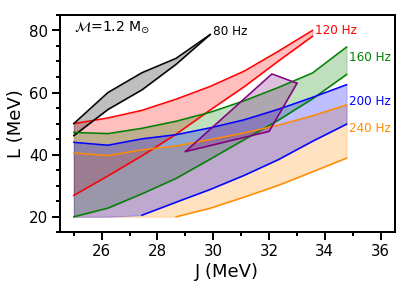
\includegraphics[width=0.45\textwidth,angle=0]{JL_spread_due_to_Ksym_grid.png}
\caption{Spread in the $J,L$ contours due to the range of $K_{\rm sym}$ values. The upper bound is for K=40 MeV, and the lower bound is for K=-200 MeV.}
\label{fig:constraints}
\end{figure}

\hspace{\parindent}Figure \ref{fig:all_constraints} shows the combination of the spread in frequency due to $t_{\rm res}$ and the spread in $L$ due to the range of $K_{\rm sym}$ values used. This figure shows the most conservative estimate of the $J$, $L$ constraints, with the upper bounds using $f\rightarrow f-\delta f$ Hz and $K_{\rm sym}=40$ MeV, and the lower bounds using $f\rightarrow f+\delta f$ Hz and $K_{\rm sym}=-200$ MeV. The ranges shown in this figure are slightly different to figure \ref{fig:constraints}, but the main uncertainty is the $K_{\rm sym}$ range.




%figure that combines all uncertainties (K_sym value, NS mass, t_res range), explain this one in text.
\begin{figure}
\centering
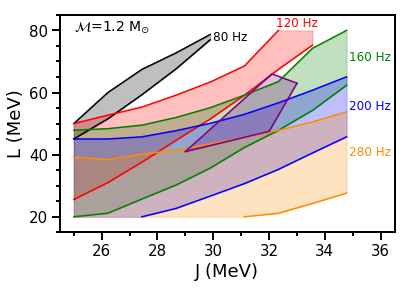
\includegraphics[width=0.45\textwidth,angle=0]{JL_spread_due_to_Ksym_and_df_grid_280.png}
\caption{Combines the ranges from figures \ref{fig:t_res_spread} and \ref{fig:constraints}.}
\label{fig:all_constraints}
\end{figure}















%%%%%%%%%%%%%%%%%%%% REFERENCES %%%%%%%%%%%%%%%%%%

% The best way to enter references is to use BibTeX:

\bibliographystyle{mnras}
\bibliography{example} % if your bibtex file is called example.bib


% Alternatively you could enter them by hand, like this:
% This method is tedious and prone to error if you have lots of references
%\begin{thebibliography}{99}
%\bibitem[\protect\citeauthoryear{Author}{2012}]{Author2012}
%Author A.~N., 2013, Journal of Improbable Astronomy, 1, 1
%\bibitem[\protect\citeauthoryear{Others}{2013}]{Others2013}
%Others S., 2012, Journal of Interesting Stuff, 17, 198
%\end{thebibliography}

%%%%%%%%%%%%%%%%%%%%%%%%%%%%%%%%%%%%%%%%%%%%%%%%%%

%%%%%%%%%%%%%%%%% APPENDICES %%%%%%%%%%%%%%%%%%%%%

\appendix

\section{Some extra material}

If you want to present additional material which would interrupt the flow of the main paper,
it can be placed in an Appendix which appears after the list of references.

%%%%%%%%%%%%%%%%%%%%%%%%%%%%%%%%%%%%%%%%%%%%%%%%%%


% Don't change these lines
\bsp	% typesetting comment
\label{lastpage}
\end{document}

% End of mnras_template.tex
